\documentclass{article}
\usepackage{graphicx} % Required for inserting images
\usepackage[top=0.9in, bottom=1in, left=1.5in, right=1.5in]{geometry}
\usepackage[utf8]{inputenc}
\usepackage[icelandic]{babel}
\usepackage[T1]{fontenc}
\usepackage[sc]{mathpazo}
\usepackage[parfill]{parskip}
% Tables and lists
\usepackage{booktabs,tabularx}
\usepackage{multirow}
\usepackage{enumerate}
\usepackage{adjustbox}
\usepackage{multicol}
\usepackage{xcolor}
\usepackage{algpseudocode}
\usepackage{tikz}
\usetikzlibrary{arrows, positioning, calc}

% Math
\usepackage{amsmath, amsfonts, amssymb, amsthm}
% Graphics

\usepackage{graphicx}
\usepackage{tikz}
% Code environment
\usepackage{minted}
%\usepackage{bm}
%\usepackage{siunitx}
%\usepackage{animate}
%\usepackage{hyperref}
%\usepackage{movie15}
%\usepackage{multicol}
%\usepackage{changepage}
\title{Tol2 Heimadæmi 3}
\author{Ragnar Björn Ingvarsson, rbi3}


\begin{document}
	
	\maketitle
	
	\section{}
	\begin{itemize}
		\item[a)] Reiknirit með vaxtargráðu $\theta(NlogN)$ myndi líta einhvernveginn svona út:
		
		\begin{algorithmic}
			\State \underline{\textbf{ParasummaFast} (long[] $A$, long[] $B$, long $K$)}
			
			\State $Sort(B)$
			\For{$i=0$ in $A$}
				\If{$BinarySearch(B$, $K-A[i]) \geq 0$}
					\State \Return true
				\EndIf
			\EndFor
			\State \Return false
		\end{algorithmic}
		
		Við sjáum útfrá þessu reikniriti að nokkrar aðgerðir eru gerðar. Við erum fyrst með $Sort$ sem raðar stökum $B$ í hækkandi röð. $Sort$ sem við ætlum að nota í java heitir Arrays.sort og hefur tímaflækjuna $\theta(NlogN)$. Síðan kemur $for$ lykkja sem gengur $N$ sinnum þar sem $A$ er af lengd $N$, þess vegna er tímaflækja $for$ lykkjunnar $O(N)$. Í hvert skipti sem $for$ lykkjan gengur í gegn framkvæmum við $BinarySearch$ sem er reiknirit sem hefur tímaflækjuna $\theta(logN)$ og þá sést að bæði $Sort$ og restin hefur tímaflækjuna $O(NlogN)$. Þess vegna er tímaflækjan fyrir reikniritið í heild sinni $\theta(NlogN)$.

		\item[b)] 
		
		\begin{verbatim}
			public static boolean nlognSumma(long[] A, long[] B, long K) {
			    Arrays.sort(B);
			    for (int i = 0; i < A.length; i++) {
			        if (Arrays.binarySearch(B, K-A[i]) >= 0) return true;
			    }
			    return false;
			}
		\end{verbatim}
		
		Þessi útfærsla fær þessar niðurstöður:
		\begin{center}
			$10000$, tími: $0.009$
			
			$20000$, tími: $0.013$, hlutfall: $1.44$
			
			$40000$, tími: $0.021$, hlutfall: $1.62$
			
			$80000$, tími: $0.048$, hlutfall: $2.29$
			
			$160000$, tími: $0.064$, hlutfall: $1.33$
			
			$320000$, tími: $0.099$, hlutfall: $1.55$

			$640000$, tími: $0.208$, hlutfall: $2.10$
			
			$1280000$, tími: $0.343$, hlutfall: $1.65$
			
			$2560000$, tími: $0.618$, hlutfall: $1.80$
		\end{center}
		
		Niðurstöðurnar eru ekki mjög nákvæmar en við sjáum að tvöföldunarhlutfallið er rúmlega $1.7$.
		
	\end{itemize}
	
	\section{}
	
	\begin{itemize}
		\item[a)] Reikniritið fyrir þetta myndi vera svona:
		
		\begin{algorithmic}
			\State $Sort(A)$1
			\State $a \gets A[1]-A[2]$
			\For{$i=2$ in $A$}
				\If{$|A[i]-A[i-1]| < a$}
					\State $a=|A[i]-A[i-1]|$
				\EndIf
			\EndFor
			\State \Return $a$
		\end{algorithmic}
		

		Við sjáum hér að $Sort$ er aftur með tímaflækju $\theta(NlogN)$ og $for$ lykkjan gengur $N-2$ sinnum og gerir constant fjölda aðgerða í hvert sinn svo tímaflækja allrar $for$ lykkjunnar er $\theta(N)$ þannig að heildar-tímaflækjan er $\theta(NlogN)$
		
		\item[b)]
		
		
		
		\begin{verbatim}
			public static void main(String[] args) {
			    int N = Integer.parseInt(args[0]);
			    double[] A = new double[N];
				
			    // Búa til slembigildi í fylkið
			    for (int i=0; i<N; i++) {
			        A[i] = StdRandom.uniformDouble()*N;
			    }
				
			    Arrays.sort(A);
			    double a = A[1]-A[0];
			    double fyrstaStak=0;
			    double annadStak=0;
			    for (int i = 2; i < A.length; i++) {
			        if (Math.abs(A[i]-A[i-1]) < a) {
			            a=A[i]-A[i-1];
			            fyrstaStak=A[i-1];
			            annadStak=A[i];
			    \textbf{}    }
			    }
			    System.out.println(Arrays.toString(A));
			    System.out.println("MinDiff: " + a);
			    System.out.println("Fyrra Stak: " + fyrstaStak)
			}
		\end{verbatim}
		
		Hér er svo mynd af keyrslu með $N=10$:
	\end{itemize}
	
	\section{}
	\begin{itemize}
		\item[a)] Hér sést að við erum með tvær $for$ lykkjur, eina ytri og eina innri. Sú ytri rennur í gegn $N-10$ sinnum og í hvert skipti sem það gerist rennur sú innri í gegn $i^2$ sinnum. Þegar við erum komin á síðasta snúning ytri lykkjunnar er $i=N-1$ og því rennur innri lykkjan í gegn $(N-1)^2$ sinnum og því fæst að tímaflækja er $\theta(N*N^2)=\theta(N^3)$.
		\item[b)] Hér erum við aftur með tvær $for$ lykkjur, eina innri og eina ytri. Við fyrstu sýn virðist eins og við viljum margfalda saman tímaflækjurnar frá báðum lykkjunum en það gengur ekki í þessu tilfelli því innri lykkjan er beint háð þeirri ytri.
		
		Við getum tekið eftir í staðinn að summan $s$, með því að prófa gildi á $N$ og ganga nokkur skref í gegn, er á forminu $2^0+2^1+2^2+2^3+...M$, $M<N$. Þess vegna sést að $s$ er rúmlega $2N$ svo tímaflækjan er $\theta(N)$.
		\item[c)] Við sjáum að hér er ein $while$ lykkja sem hækkar $i$ um einn og bætir $i$ við $s$ í hvert skipti. Lykkjan er háð $s$, svo við fáum að $s=\frac{i(i+1)}{2}$ á meðan $s<=N$. Við getum þá fundið rúmlega tímaflækju forritsins með því að leysa rúmlega fyrir $i$ til að komast eins nálægt $N$ í jöfnunni $\frac{i(i+1)}{2}<N \Rightarrow \frac{i^2+i}{2}<N$ en hér sést að fyrir háar tölur skiptir $i$ engu máli þar sem $i^2$ er einnig í dæminu, og við hendum út $\frac{1}{2}$ líka og fáum $i^2<N$ og því hlýtur $i \approx \sqrt[]{N}$ svo tímaflækjan er $\theta(\sqrt{N})$
	\end{itemize}
	\newpage
	\section{}
	
	\begin{itemize}
		\item[a)] $3, 5, 6, 3, 3, 2, 2$
		
		Við erum semsagt með röð af lengd 7 frá 0-6 og sjáum að eftirfarandi tengingar eru gefnar:
		
		\[0-3\]\[1-5\]\[2-6\]\[3-3\]\[4-3\]\[5-2\]\[6-2\]
		
		Hér sést um leið að þessi runa er ólögleg þar sem $2$ tengist við $6$ og $6$ tengist líka við $2$. Þar með myndast lykkja og engin rót fæst fyrir $2$ og $6$.
		
		\begin{center}
		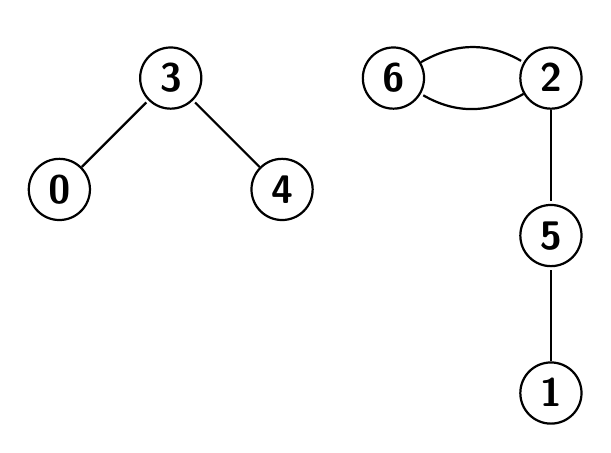
\begin{tikzpicture}[>=stealth',shorten >=1pt,auto,node distance=2cm,
			thick,main node/.style={circle,draw,font=\sffamily\Large\bfseries}]
			
			\node[main node] (3) {3};
			\node[main node] (0) [below left of=3] {0};
			\node[main node] (4) [below right of=3] {4};
			\node[main node] (6) [above right of=4] {6};
			\node[main node] (2) [right of=6] {2};
			\node[main node] (5) [below of=2] {5};
			\node[main node] (1) [below of=5] {1};
			
			\path[every node/.style={font=\sffamily\small}]
			
			(0) edge node {} (3)
			(4) edge node {} (3)
			(2) edge node {} (5)
			(2) edge[bend left] node {} (6)
			(6) edge[bend left] node {} (2)
			(1) edge node {} (5);
		\end{tikzpicture}
		\end{center}
		
		Þetta af sjálfsögðu getur ekki birst í vigtuðu \textit{Quick-union} því það er ólöglegt.
		\item[b)] $0,2,2,2,0,2,2$
		
		Hér myndast tengingarnar: 
		
		\[0-0\]\[1-2\]\[2-2\]\[3-2\]\[4-0\]\[5-2\]\[6-2\]
		
		Hér myndast engar lykkjur og sést að $0$ og $2$ eru rætur svo myndin lítur svona út:
		
		\begin{center}
		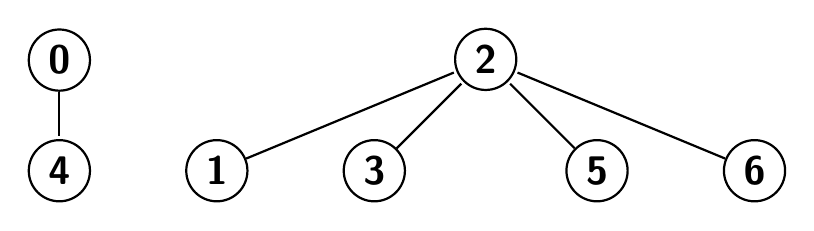
\begin{tikzpicture}[>=stealth',shorten >=1pt,auto,node distance=2cm,
		thick,main node/.style={circle,draw,font=\sffamily\Large\bfseries}]
		
		\node[main node] (0) {0};
		\node[main node] (4) [below=0.6cm of 0] {4};
		\node[main node] (1) [right of=4] {1};
		\node[main node] (3) [right of=1] {3};
		\node[main node] (2) [above right of=3] {2};
		\node[main node] (5) [below right of=2] {5};
		\node[main node] (6) [right of=5] {6};
		
		\path[every node/.style={font=\sffamily\small}]
		
		(0) edge node {} (4)
		(1) edge node {} (2)
		(3) edge node {} (2)
		(5) edge node {} (2)
		(6) edge node {} (2);
		\end{tikzpicture}
		\end{center}
		
		Þetta er löglegt því allar tengingar eru innan marka og engar lykkjur hafa myndast, og einnig eru allar tölur með rót. Þetta getur líka birst í vigtuðu \textit{Quick-union} með aðgerðunum: $(0,4),(2,1),(2,3),(2,5),(2,6)$
		
		\item[c)] $4,0,2,0,4,4,3$
		
		\[0-4\]\[1-0\]\[2-2\]\[3-0\]\[4-4\]\[5-4\]\[6-3\]
		
		Hér sést að $2$ og $4$ eru rætur og myndin lítur þá svona út:
		
		\begin{center}
			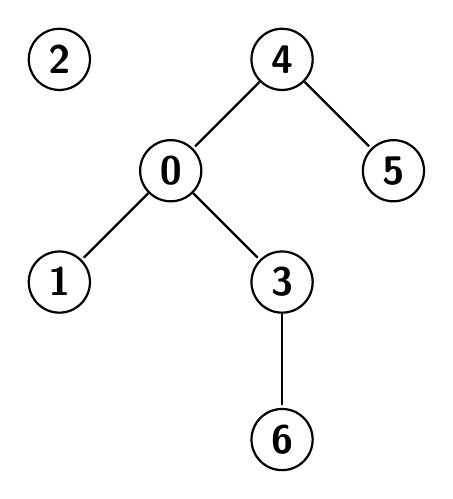
\begin{tikzpicture}[>=stealth',shorten >=1pt,auto,node distance=2cm,
				thick,main node/.style={circle,draw,font=\sffamily\Large\bfseries}]
				
				\node[main node] (4) {4};
				\node[main node] (0) [below left of=4] {0};
				\node[main node] (5) [below right of=4] {5};
				\node[main node] (1) [below left of=0] {1};
				\node[main node] (3) [below right of=0] {3};
				\node[main node] (6) [below of=3] {6};
				\node[main node] (2) [above left of=0] {2};
				
				\path[every node/.style={font=\sffamily\small}]
				
				(4) edge node {} (5)
				(4) edge node {} (0)
				(0) edge node {} (1)
				(0) edge node {} (3)
				(3) edge node {} (6);
			\end{tikzpicture}
		\end{center}
		
		Þetta er lögleg uppsetning skv. reglunum sem ég benti á í b) en hins vegar getur þetta ekki birst í vigtuðu \textit{Quick-union} því við sjáum að dýpt fylkisins er $3$ en $\log_2(7)\approx2.8$. Þetta má ekki því dýpt vigtaðs \textit{Quick-union} má ekki vera meiri en $\log_2(N)$ þar sem $N$ er fjöldi staka.
	\end{itemize}
	
	\section{} Við byrjum með $0,1,2,3,4$ og fáum:
	
	\begin{center}
		
\begin{tikzpicture}[>=stealth',shorten >=1pt,auto,node distance=2cm,
			thick,main node/.style={circle,draw,font=\sffamily\Large\bfseries}]
			
			\node[main node] (0) {0};
			\node[main node] (1) [right of=0] {1};
			\node[main node] (2) [right of=1] {2};
			\node[main node] (3) [right of=2] {3};
			\node[main node] (4) [right of=3] {4};
		
		\end{tikzpicture}
	\end{center}
	
	Síðan gerist $union(0,1)$ og fæst þá:
	
	\begin{center}
		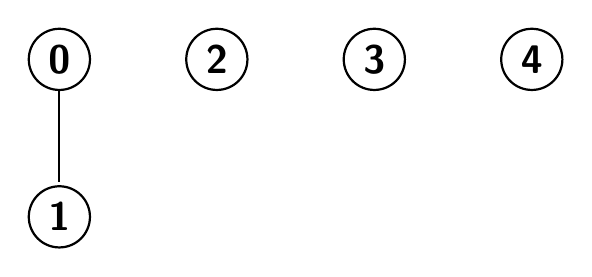
\begin{tikzpicture}[>=stealth',shorten >=1pt,auto,node distance=2cm,
			thick,main node/.style={circle,draw,font=\sffamily\Large\bfseries}]
			
			\node[main node] (0) {0};
			\node[main node] (1) [below of=0] {1};
			\node[main node] (2) [right of=0] {2};
			\node[main node] (3) [right of=2] {3};
			\node[main node] (4) [right of=3] {4};
			
			\path[every node/.style={font=\sffamily\small}]
			(0) edge node {} (1);
		\end{tikzpicture}
	\end{center}
	
	Næst gerist $union(3,1)$ og þar sem við erum að nota vigtað \textit{Quick-union} þá finnum við rót $1$ sem er $0$ og þar sem $0$ tréð er þyngra en $3$ þá tengist $3$ beint við rótina:
	
	\begin{center}
		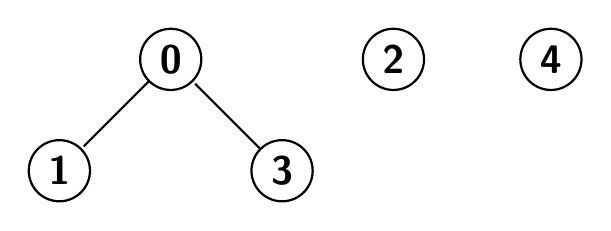
\begin{tikzpicture}[>=stealth',shorten >=1pt,auto,node distance=2cm,
			thick,main node/.style={circle,draw,font=\sffamily\Large\bfseries}]
			
			\node[main node] (0) {0};
			\node[main node] (1) [below left of=0] {1};
			\node[main node] (3) [below right of=0] {3};
			\node[main node] (2) [above right of=3] {2};
			\node[main node] (4) [right of=2] {4};
			
			\path[every node/.style={font=\sffamily\small}]
			(0) edge node {} (1)
			(3) edge node {} (0);
		\end{tikzpicture}
	\end{center}
	
	Síðan $union(2,4)$:
	
	\begin{center}
		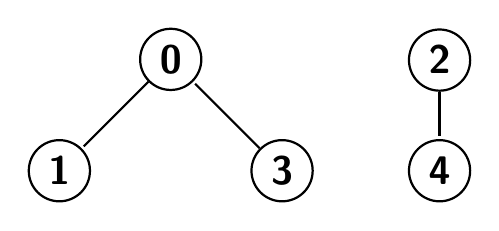
\begin{tikzpicture}[>=stealth',shorten >=1pt,auto,node distance=2cm,
			thick,main node/.style={circle,draw,font=\sffamily\Large\bfseries}]
			
			\node[main node] (0) {0};
			\node[main node] (1) [below left of=0] {1};
			\node[main node] (3) [below right of=0] {3};
			\node[main node] (4) [right of=3] {4};
			\node[main node] (2) [above=0.6cm of 4] {2};
			
			\path[every node/.style={font=\sffamily\small}]
			(0) edge node {} (1)
			(2) edge node {} (4)
			(3) edge node {} (0);
		\end{tikzpicture}
	\end{center}
	
	Og loks $union(4,1)$ sem finnur rætur beggja stakanna, sem eru þá $0$ og $2$, og við sjáum að þar sem $2$ er léttari þá sameinast $2$ við $0$ og til að minnka dýpt þá tengist $4$ einnig við $0$ og við fáum:
	\begin{center}
	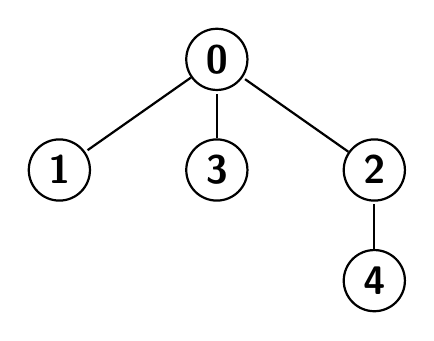
\begin{tikzpicture}[>=stealth',shorten >=1pt,auto,node distance=2cm,
		thick,main node/.style={circle,draw,font=\sffamily\Large\bfseries}]
		
		\node[main node] (1) {1};
		\node[main node] (3) [right of=1] {3};
		\node[main node] (0) [above=0.6cm of 3] {0};
		\node[main node] (2) [right of=3] {2};
		\node[main node] (4) [below=0.6cm of 2] {4};
		
		\path[every node/.style={font=\sffamily\small}]
		(0) edge node {} (1)
		(3) edge node {} (0)
		(4) edge node {} (2)
		(2) edge node {} (0);
		
	\end{tikzpicture}
\end{center}



Að lokum fæst þá $id$-ið $0,0,0,0,2$.
	
	
\end{document}























